\section{Einleitung}
	\label{sec:einleitung}
	
	Lichstrahlen werden beim "Ubergang von einem Material in ein anderes Gebrochen.
	Dies liegt an der "Anderung der materialabh"angigen Phasengeschwindigkeit.
	In diesem Versuch wird die Brechung an einer oder zwei Linsen genauer untersucht.

\section{Theorie}
	\label{sec:theorie}

	Linsen bestehen aus einem Material, welches optisch dichter ist als Luft.
	Je nach Form besitzen diese spezielle Eigenschaften.
	
	\begin{figure}[htbp]
		\centering
		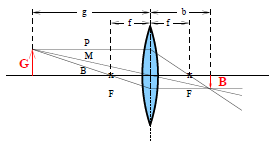
\includegraphics[width = 12cm]{img/sammellinse.PNG}
		\caption{Abbildung einer d"unnen Sammellinse, einer Zerstreuungslinse und einer dicken Sammellinse und deren optischen Eigenschaften \cite{anleitung}}
		\label{sammellinse}
	\end{figure}

	\begin{center}
			\tiny{Brennweite $f$, Brennpunkt $F$, Bildweite $b$, Gegenstandsweite $g$, Gegenstandsgr"o"se $G$, Bildgr"o"se $B$, Parallelstrahl $P$, Mittelpunktstrahl $M$, Brennpunktstrahl $B$}
	\end{center}

	\subsection{Linsen} % (fold)
	\label{sub:sammellinse}
	
	Die Sammellinse ist in der Mitte dick und wird zu den Enden d"unner. Dadurch b"undeln diese das Licht im Brennpunkt.
	Brennweite $f$ und Bildweite $b$ sind positiv und es entsteht ein reelles Bild.

	Bei der Zerstreuungslinse sind Brennweite $f$ und Bildweite $b$ negativ und es entsteht ein virtuelles Bild.

	Bei dicken Linsen ist eine Reduktion bei der Brechung auf die Mittelebene nicht mehr m"oglich und es werden zwei Hauptebenen eingef"uhrt, an denen die Brechung gedacht stattfindet.

	F"ur die Beschreibung der Bildkonstruktion werden drei ausgezeichnete Strahlen verwendet:
	Parallelstrahl $P$, Mittelpunktsstrahl $M$ und Brennpunktsstrahl $B$, wie in Abb. \eqref{sammellinse} gezeigt.

	\subsection{Abbildungsgesetz} % (fold)
	\label{sub:abbildungsgesetz}
	
	Durch Strahlens"atze und aus der Bildkonstruktion ergibt sich das Abbildungsgesetz

	\begin{equation}
		V = \frac{V}{G} = \frac{b}{g}\, .
	\end{equation}

	\subsection{Linsengleichung} % (fold)
	\label{sub:linsengleichung}
	
	F"ur d"unne Linsen folgt daraus die Linsengleichung:

	\begin{equation}
		\frac{1}{f} = \frac{1}{b} + \frac{1}{g}\, .
	\end{equation}

	Bei dicken Linsen werden die Werte $b$ und $g$ jeweils von der n"aherliegenden Hauptebene an gemessen. Dadurch kann auch bei dieser die Linsengleichung angewendet werden.

	\subsection{Brechkraft} % (fold)
	\label{sub:brechkraft}
	
	Die Linsengleichung gibt gleichzeitig auch die Brechkraft $D$ der Linse wieder. F"ur die Zusammensetzung mehrerer d"unner Linsen gilt:

	\begin{equation}
		D = \frac{1}{f} = \sum_i^N D_\mathrm{i} \label{brechkraft}
	\end{equation}

	Die Brechkraft wird in Dioptrie [dpt = 1/m] gemessen.

	Haben Linsen zwei unterschiedlich gekr"ummte Fl"achen, so kann man sich diese als zwei d"unne, einseitig plane zusammengesetzte Linsen denken.
	Die Brechkraft kann nun wieder mit Gl. \eqref{brechkraft} berechnet werden.

	\subsection{Abbildungsfehler} % (fold)
	\label{sub:abbildungsfehler}

	Bei den Abbildungsfehlern gibt es die sp"ahrische und die chromatische Abberation.
	
	\subsubsection{Sp"ahrische Abberation} % (fold)
 	\label{sub:sp_ahrische_abberation}
 
  	Bei achsennahen Strahlen wird das Licht an der Linse weniger stark gebrochen als bei achsenfernen Strahlen.
  	Dadurch kommt es zu einer Verschiebung des Brennpunktes hinter der Linse.
  	Der Brennpunkt von achsenfernen Strahlen liegt n"aher an der Linse als der von achsennahen Strahlen, wodurch das Bild unscharf wird.

   Um wieder ein scharfes Bild zu erhalten, k"onnen die achsenfernen Strahlen z.B. mit einer Irisblende ausgeblendet werden.

   \subsection{chromatische Abberation} % (fold)
   \label{sub:chromatische_abberation}
   
   Licht verschiedener Wellenl"angen wird unterschiedlich stark gebrochen.
   Je k"urzer die Wellenl"ange, umso st"arker die Brechung.
   Dadurch liegt der Brennpunkt von kurzwelligem Licht (z.B. blau) n"aher an der Linse als der von langwelligem Licht (z.B. rot).

   Diese Eigenschaft des Lichts wird Dispersion genannt.
